\chapter{Annexes}\label{sec:Annexes}

\section{Required packages}\label{sec:ANNEXERequiredPackages}
Here is a list of packages used in the FA$\mu$ST project. The installation of this packages are automatically done. There are nothing to do. (see the source directory "./externals").
\begin{itemize}
\item Library \textbf{Eigen} \url{http://eigen.tuxfamily.org}: C++ template library for linear algebra: matrices, vectors, numerical solvers, and related algorithms.
\item Library \textbf{OpenBLAS} \url{http://www.openblas.net}:  Optimized BLAS library based on GotoBLAS2 1.13 BSD version.
\item Library \textbf{xml2} \url{http://xmlsoft.org}
\item Library \textbf{matio} \url{https://sourceforge.net/projects/matio}
\end{itemize}

\section{Compatibility between MATLAB and compiler gcc}\label{sec:ANNEXECompatibilityMatlabCompiler}
Adjust your version of GCC compiler in order to run the installation properly. The use of the mex function in Matlab requires that you have a third-party compiler installed on your system. The latest version of Matlab (2016a in our case) only supports up to GCC 4.7 (see \url{http://fr.mathworks.com/support/compilers/R2016a/index.html?sec=glnxa64} for more detail).
To temporally change your version of gcc compiler, you can modify the environment variable CC an CXX. For that, export your CC and CXX variables corresponding to gcc and g++ binaries path :
\begin{itemize}
\item find your gcc and g++ version path using \texttt{which} command in a terminal :
\begin{lstlisting}
> which gcc
> which g++
\end{lstlisting}

\item Open your ~/.bashrc file and save the return-path of gcc and g++ like:
\begin{lstlisting}[backgroundcolor=\color{white}]
# export version of gcc
export CC=/usr/lib64/ccache/gcc
export CXX=/usr/lib64/ccache/g++
\end{lstlisting}
\end{itemize}

An other way to change the version of compiler use by mex function from matlab command is : 
\begin{lstlisting}
> mex -setup
\end{lstlisting}


\section{Further information about Build \& Install process}\label{sec:ANNEXEInfoBuildInstall}
When using the \textbf{cmake} command to generate the build system, \textbf{cmake} performs a list of tests to determine the system configuration and manage the build system. If the configuration is correct then the build system is generated and written. In this case, the three last lines of the console log of \textbf{cmake} command should be:
\begin{lstlisting}[backgroundcolor=\color{white}]
-- Configuring done 
-- Generating done 
-- Build files have been written to: <YOUR/LOCAL/DIRECTORY/build>
\end{lstlisting}

The command \textbf{make} will compile the build files.\\

The command \textbf{sudo make install} will install the library and others components in the default directory: \\
\texttt{/usr/local/lib/libfaust.a} for the FA$\mu$ST library, \\
\texttt{\textasciitilde /Documents/MATLAB/faust/} for the wrapper matlab.\\
You must have administrator privilege because the library file \texttt{libfaust.a} is copied in an root path directory. If you do not have administrator privilege, you can realize a local install using \texttt{cmake} optional parameter \texttt{-DCMAKE\_INSTALL\_PREFIX="<Your/Install/Dir>"}. 

The \texttt{cmake} optional parameter \texttt{-DCMAKE\_INSTALL\_PREFIX="<Your/Install/Dir>"} allows to install the binaries on the selected install directory. 

The \texttt{cmake} optional parameter \texttt{-G "CodeBlocks - Unix Makefiles"} allows to generate the Code Blocks project and the Unix Makefiles.\\ 
The \texttt{cmake} optional parameter \texttt{-G "Xcode"} allows to generate the Xcode project. 




%for windows
\section{Required packages on Windows platform}\label{sec:WinRequiredPackages}
Here is a list of packages used in the FA$\mu$ST project. Eigen and OpenBlas library are automatically installed : there are nothing to do (see the directory "./externals/win/").
\begin{itemize}
\item \textbf{Eigen} is a C++ template library for linear algebra: matrices, vectors, numerical solvers, and related algorithms (see \url{http://eigen.tuxfamily.org}).
\item \textbf{OpenBLAS} is an optimized BLAS library based on GotoBLAS2 1.13 BSD version. (see \url{http://www.openblas.net}). To install OpenBlas, refer to \url{https://github.com/xianyi/OpenBLAS/wiki/Installation-Guide}. You can directly download precompiled binary here \url{https://sourceforge.net/projects/openblas/files/v0.2.14/}
\end{itemize}



\section{Add environment variable on Windows platform}\label{sec:ANNEXEEnvironmentVariableWindows}
Here is the steps to add an environment variable in Windows 7.
\begin{enumerate}
\item From the Desktop, right-click the Computer icon and select Properties. If you don't have a Computer icon on your desktop, click the Start button, right-click the Computer option in the Start menu, and select Properties.
\item Click the Advanced System Settings link in the left column.
\item In the System Properties window, click on the Advanced tab, then click the Environment Variables button near the bottom of that tab.
\item In the Environment Variables window (pictured below), highlight the Path variable in the "System variables" section and click the Edit button. Add or modify the path lines with the paths you want the computer to access. Each different directory is separated with a semicolon as shown below.
\begin{lstlisting}[backgroundcolor=\color{white}]
C:\Program Files;C:\Winnt;C:\Winnt\System32
\end{lstlisting}

\begin{figure}[!h] %%[!htbp]
\centering
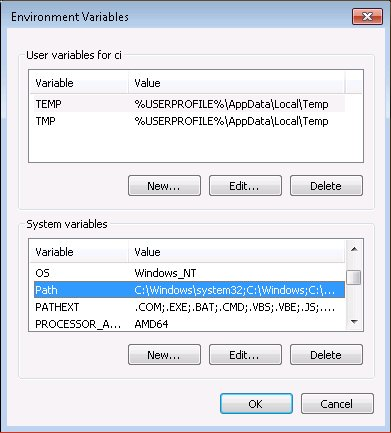
\includegraphics[scale=0.5]{images/EnvironmentVariable.jpeg}
%\caption{cmake GUI}
\label{fig:EnvironmentVariable}
\end{figure}

\end{enumerate}



